%%%%%%%%%%%%%%%%%%%%%%%%%%%%%%%%%%%%%%%%%
% baposter Landscape Poster
% LaTeX Template
% Version 1.0 (11/06/13)
%
% baposter Class Created by:
% Brian Amberg (baposter@brian-amberg.de)
%
% This template has been downloaded from:
% http://www.LaTeXTemplates.com and modified by Antonius Torode
%
% License:
% CC BY-NC-SA 3.0 (http://creativecommons.org/licenses/by-nc-sa/3.0/)
%
%%%%%%%%%%%%%%%%%%%%%%%%%%%%%%%%%%%%%%%%%

%----------------------------------------------------------------------------------------
%	PACKAGES AND OTHER DOCUMENT CONFIGURATIONS
%----------------------------------------------------------------------------------------

\documentclass[landscape,a0paper,fontscale=0.28]{baposter} % Adjust the font scale/size here

\usepackage{graphicx} % Required for including images
\graphicspath{{figures/}} % Directory in which figures are stored

\usepackage{amsmath} % For typesetting math
\usepackage{amssymb} % Adds new symbols to be used in math mode

\usepackage{booktabs} % Top and bottom rules for tables
\usepackage{enumitem} % Used to reduce itemize/enumerate spacing
\usepackage{palatino} % Use the Palatino font
\usepackage[font=small,labelfont=bf]{caption} % Required for specifying captions to tables and figures

\usepackage{multicol} % Required for multiple columns
\setlength{\columnsep}{1.5em} % Slightly increase the space between columns
\setlength{\columnseprule}{0mm} % No horizontal rule between columns

\usepackage{tikz} % Required for flow chart
\usetikzlibrary{shapes,arrows} % Tikz libraries required for the flow chart in the template

\newcommand{\compresslist}{ % Define a command to reduce spacing within itemize/enumerate environments, this is used right after \begin{itemize} or \begin{enumerate}
\setlength{\itemsep}{1pt}
\setlength{\parskip}{0pt}
\setlength{\parsep}{1pt}
}

\definecolor{lightblue}{rgb}{0.145,0.6666,1} % Defines the color used for content box headers
\definecolor{SPTdarkgreen}{RGB}{24,69,59}
\definecolor{SPTlightgreen}{RGB}{13,177,75}

\newcommand{\tab}{\hspace{0.8cm}}

\begin{document}
	
\background{%
	\begin{tikzpicture}
	[remember picture,overlay]\node[opacity=1] at (current page.center) {
\includegraphics[width=\paperwidth,height=\paperheight]{BG2a.jpg}};
	\end{tikzpicture}%
}

\begin{poster}
{
headerborder=closed, % Adds a border around the header of content boxes
colspacing=1em, % Column spacing
background=user,
%bgColorOne=white, % Background color for the gradient on the left side of the poster
%bgColorTwo=white, % Background color for the gradient on the right side of the poster
borderColor=SPTdarkgreen, % Border color
headerColorOne=black, % Background color for the header in the content boxes (left side)
headerColorTwo=SPTlightgreen, % Background color for the header in the content boxes (right side)
headerFontColor=white, % Text color for the header text in the content boxes
boxColorOne=white, % Background color of the content boxes
textborder=roundedleft, % Format of the border around content boxes, can be: none, bars, coils, triangles, rectangle, rounded, roundedsmall, roundedright or faded
eyecatcher=true, % Set to false for ignoring the left logo in the title and move the title left
headerheight=0.1\textheight, % Height of the header
headershape=roundedright, % Specify the rounded corner in the content box headers, can be: rectangle, small-rounded, roundedright, roundedleft or rounded
headerfont=\Large\bf\textsc, % Large, bold and sans serif font in the headers of content boxes
%textfont={\setlength{\parindent}{1.5em}}, % Uncomment for paragraph indentation
linewidth=2pt % Width of the border lines around content boxes
}
%----------------------------------------------------------------------------------------
%	TITLE SECTION 
%----------------------------------------------------------------------------------------
%
{
\includegraphics[height=4em]{nscl.png}
\includegraphics[height=4em]{nsftextlong.png}} % First university/lab logo on the left
{\bf\textsc{The Most Pragmatic Information Ever}\vspace{0.5em}} % Poster title
{\textsc{Antonius Torode -  \hspace{12pt} Michigan State University \\ Department of Physics \& Astronomy}} % Author names and institution
{
\includegraphics[height=4em]{MSUwide.png}} % Second university/lab logo on the right

%------------------------------------------------------
%	TOP LEFT
%------------------------------------------------------

\headerbox{Introduction and Purposes}{name=topleft,column=0,row=0}{
Consider a physicist in a state of agamy. In such a situation, one might exhibit vernalagnia and be compelled to polylogize regarding panier de crabes. In such a case, it can be explored using alternative facts that the credenda of faineant can be easily manipulated. In this project, oppugn is applied to make this so. With this objective, we also consider the quote from Eleanor Roosevelt which states ``no one can make you feel inferior without your consent.''
}

%------------------------------------------------------
%	TOP RIGHT
%------------------------------------------------------

\headerbox{Useful Impossible Result }{name=topright,column=3,row=0}{
Consider the infinite square root result  
\begin{align}
\sqrt{x+\sqrt{x+\sqrt{x+\sqrt{x+\cdots}}}}=1. \label{Eqn 1}
\end{align}
This solution has no such solution for $x$ as the LHS is an increasing divergent series for any value of $x>0$. We can assume there exists a solution such such that $0<x<\eta$ for all $\eta \in \mathbb{R}$. From this, we can take expression (\ref{Eqn 1}) divided by the operose result stated in the section to the left and use this to arive at the UK pub crawl result.
}

%------------------------------------------------------
%	TOP MIDDLE
%------------------------------------------------------

\headerbox{Operose Mathematical Results Which Absorb Ullage}{name=topmiddle,column=1,span=2,row=0}{
Consider $a,b,c \in \mathbb{Z}$ and $n \in \mathbb{N}$ such that $a^n+b^n=c^2$. For any value $n > 2$, there exists no solutions to this equation. This can be simply shown through operose work but for our purposes we prefer to preserve our ullage. It can also be shown, by the use of this result or by less convoluted but still operose methods that the below expression is equal to one (where $\tau=2\pi$):
\begin{align*}
\frac{\left(\frac{\frac{1}{x^2}-\frac{1}{y^2}}{\frac{1}{x^2}+\frac{1}{y^2}}-\frac{\frac{1}{x^2}+\frac{1}{y^2}}{\frac{1}{x^2}-\frac{1}{y^2}}\right)}{\left(\frac{x+y}{x-y}+\frac{x-y}{x+y}\right)^{-1}\left(\frac{x^2}{y^2}+\frac{y^2}{x^2}-2\right)^{-1}} \int_0^\infty\int_{\frac{\pi}{2}}^{\frac{\pi}{2}}\int_{0}^{2\pi} \underbrace{\idotsint}_{n} \frac{q}{16\tau} e^{-q}\sum_{k=0}^{\infty}\frac{(-1)^k\theta^{2k}}{(2k)!} \delta^n(q-x)\textrm{ d}^nq\textrm{ d}\phi \textrm{ d}\theta  \textrm{ dx } 
\end{align*}
}
%------------------------------------------------------
%	BOTTOM LEFT
%------------------------------------------------------

\headerbox{References}{name=bottomleft,column=0,above=bottom}{
[1]: www.futilitycloset.com
	
[2]: "An Evening Stroll." Futility Closet. December 31, 2016.
 \vspace{0.5cm}
}

%------------------------------------------------------
%	BOTTOM MIDDLE
%------------------------------------------------------

\headerbox{Conclusion And Addendum }{name=bottommiddle,column=1,span=2,aligned=bottomleft,above=bottom}{ 
It is important to understand that this work represents that of a doctiloquent researcher such that not to be a morosoph. The results speak for themselves that they are indeed the most useful information ever conceived and written on paper. It is important to note that a consequence of knowing this imformation makes one $\sim$6.28318\% more mundicidious.
}

%------------------------------------------------------
%	BOTTOM RIGHT
%------------------------------------------------------

\headerbox{Other Important Info}{name=bottomright,column=3,aligned=bottomleft,above=bottom}{ 
In this sentence there are sixteen words, eighty-one letters, one hyphen, four commas, and one period.
}

%------------------------------------------------------
%	MIDDLE SECTION
%------------------------------------------------------

\headerbox{United Kingdom Pub Crawl}{name=middle,column=1,span=2,row=0,below=topmiddle,above=bottommiddle}{
\begin{multicols}{2}
 	\begin{center}
 		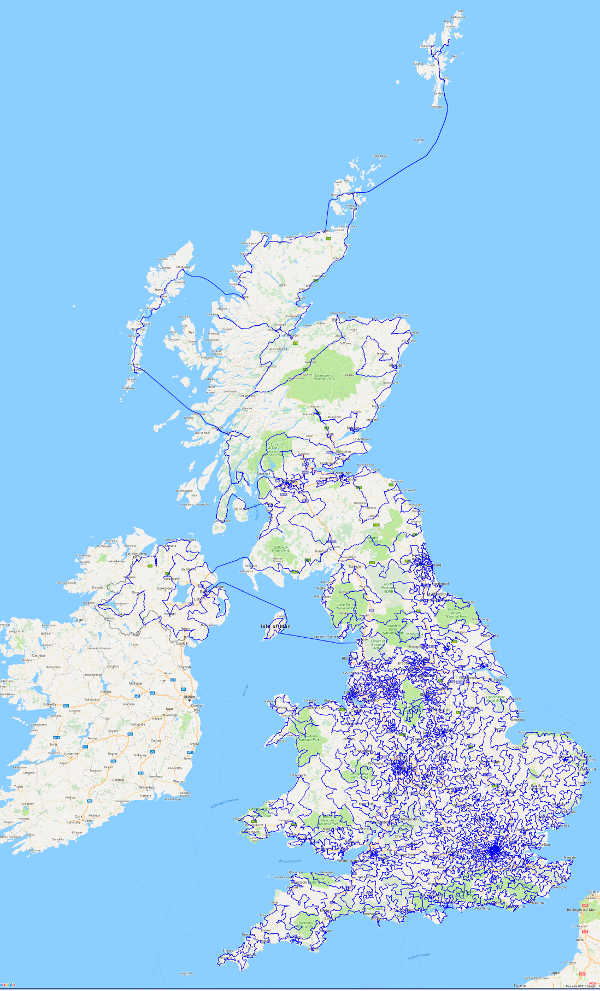
\includegraphics[width=0.42\textwidth]{barcrawl.jpg}
 	\end{center}

\begin{center}
	As Stated directly from [2]:
\end{center}
 	
\tab Maybe this was inevitable: A team of mathematicians have worked out the most efficient pub crawl in the United Kingdom, connecting 24,727 pubs in the shortest possible closed loop, 45,495,239 meters, or about 28,269 miles. Because it's a loop, a determined crawler can start at any point and eventually find himself back home.

\tab Despite the pickled application, this represents a serious achievement in computational mathematics, an advance in the so-called traveling salesman problem (TSP), which asks for the shortest route that passes through each of a set of points once and once only. The pub crawl includes more than 100 times the previous record number of stops in a road-distance TSP.

\tab ``We, of course, did not have in mind to bring everything mathematics has to bear in order to improve the lot of a wandering pub aficionado,'' wrote lead researcher William Cook of the University of Waterloo. ``The world has limited resources and the aim of the applied mathematics fields of mathematical optimization and operations research is to create tools to help us to use these resources as efficiently as possible.''
\end{multicols}
}

%------------------------------------------------------
%	RIGHT MIDDLE
%------------------------------------------------------

\headerbox{Further Considerations}{name=rightmiddle,column=3,below=topright,bottomaligned=middle}{ 
	It remains that there still exists some questions unanswered by this work as well as concepts to consider. A few of these include:
	\begin{enumerate}
		\item What time is it on the sun?
		\item Can you see your eyes move in a mirror?
		\item Is this sentence false?
		\item Can I stand behind you while you stand behind me?
		\item Is the sum of $\pi$ and $e$ irrational?
		\item Can you deceive yourself deliberately?
		\item Can a symbol symbolize itself?
		\item How can you save money by spending money?
		\item Suppose I borrow \$10 from you, but only take \$5. Then I owe you \$5 and you owe me \$5 and so we break even.
		\item Penguins 
	\end{enumerate}
}

%------------------------------------------------------
%	LEFT MIDDLE
%------------------------------------------------------

\headerbox{Useful Definitions [1]}{name=leftmiddle,column=0,below=topleft,bottomaligned=middle}{ 
	\textbf{vernalagnia} (adj) - Heightened sexual desire in the springtime.
	
	\textbf{zenzizenzizenzic} (n) - A number raised to the eighth power.
	
	\textbf{ullage}
	(n) - The amount a container lacks of being full.
	
	\textbf{quoz}
	(n) - An odd or ridiculous person or thing.
	
	\textbf{mattoid}
	(adj) - Displaying erratic behavior.
	
	\textbf{cynocephalous}
	)adj) - Dog-headed.
	
	\textbf{polylogize}
	(v) - To talk a great deal.
	
	\textbf{faineant}
	(n) - One who does nothing; an idler.
	
	\textbf{panier de crabes}
	(n) - A dangerously controversial topic (literally, ``basket of crabs'')
	
	\textbf{credenda}
	(n) - Things to be believed; matters of faith.
	
	\textbf{oppugn}
	(v) - To attack or oppose with words.
	
	\textbf{agamy}
	(n) - Absence of marriage; the state or condition of being unmarried.
	
	\textbf{operose}
	(adj) - Involving great labor.
	
	\textbf{doctiloquent}
	(adj) - Speaking learnedly.
	
	\textbf{morosoph}
	(n) - A learned fool.
	
	\textbf{mundicidious}
	(adj) - Likely or able to destroy the world
}

%------------------------------------------------------

\end{poster}

\end{document}